\documentclass[aps,prc,reprint,amsmath,nofootinbib]{revtex4-1}

\usepackage{hyperref}
\usepackage{graphicx}
\usepackage{subcaption}
\usepackage{tabularx}
\graphicspath{{fig/}}

%\usepackage{tikz}
%\usetikzlibrary{shapes,calc,matrix}

%\usepackage{mdwlist}
%\renewcommand\labelitemi{\raisebox{.3ex}{\tiny$\bullet$}}

%\newcommand{\trento}{T\raisebox{-.5ex}{R}ENTo}
%\newcommand{\nch}{N_\text{ch}}
%\newcommand{\eccratio}{\sqrt{\langle \varepsilon_2^2 \rangle}/\sqrt{\langle \varepsilon_3^2 \rangle}^{\,0.6}}

\begin{document}

\title{Entropy deposition in ultra-relativisitic nucleus-nucleus collisions}

\author{J.\ Scott Moreland}
\date{\today}

\maketitle

\section{Introduction}

Microseconds after the big bang, our universe was super heated to several trillion kelvin. In these extreme conditions, nuclear matter existed as a hot 
soup of deconfined quarks and gluons. As the universe expanded and cooled, these colored degrees of freedom recombined to form colorless hadrons 
(e.g. protons) and kickstarted the elaborate process of nucleosysnthesis \cite{Heinz:2004qz}.

Evidence for this high temperature phase of deconfined nuclear matter was first provided by researchers at the Relativisitic Heavy-Ion Collider (RHIC) 
in Brookhaven, NY. Collisions of ultra-relativistic gold nuclei at RHIC produced hot and dense fireballs that exhibited strong signs of collective flow 
\cite{Adams:2005dq}. These flow results were significantly stronger than those of lower energy nuclear collisions at the Super Proton Synchrotron (SPS) 
\cite{Shuryak:2004cy}. This energy dependent growth in collectivity led RHIC scientists to announce indirect evidence for a new state of deconfined nuclear 
matter dubbed the quark-gluon plasma (QGP) \cite{BNL}.

The large flow signals observed at RHIC supported a \emph{strongly} coupled QGP liquid and upended wide expectations that high temperature nuclear matter 
would exhibit small coupling $\alpha_s(p~T) \ll 1$ and behave like a weakly interacting gas \cite{Shuryak:2004cy}. Relativistic fluid dynamic simulations which modeled 
the produced fireball using distinct liquid and gaseous phases to describe the strongly coupled QGP liquid and weakly coupled hadron gas were highly successful in 
explaining the anomalous flow behaviour observed in the data and established the hydrodynamic nature of hot and dense nuclear matter \cite{Kolb:2003dz}.

The success of these first hydrodynamic simulations, which did not account for viscosity, suggested that the QGP was nearly inviscid. In fact, ideal hydrodynamics 
worked so well in describing the evolution of relativistic heavy-ion collisions that the QGP was called the ``perfect fluid''. It has since become a task of great 
interest to extract the thermodynamic and transport properties of the QGP droplet produced in relativistic heavy-ion collisions, as such properties shed light on
exotic regions of the nuclear phase diagram and improve our murky understanding of primordial matter in the big bang.

Fundamental QGP properties are extracted from computer simulations using a process known as model to data comparison. Theoretical guidance is used to construct
realistic, albeit under constrained, hydrodynamic models for the full spacetime evolution of the produced fireball. These models generate events exactly as they might
occur inside the detector and output moc experimental data. By comparing the model's moc data to experimental data, free parameters of the model are constrained. Such 
model to data comparisons thus provide valuable access to fundamental properties of the short lived QGP fireball which cools too quickly (${\sim}10^{-23}$ s) to be 
observed directly.

In order to extract these properties accurately, it's important that the model admit a faithful description of reality. In this report we concentrate on improving 
initial condition models used to describe the deposition of entropy in the hydrodynamic standard model. The veracity of these initial conditions governs the 
predictive power of hydrodynamic model to data comparisons and consequently our understanding of fundamental QGP properties.
  
\section{Relativistic nuclear collisions}

Before talking about the specifics of hydrodynamic initial conditions and why they are important to QGP parameter extractions, it's useful to take a step back 
and discuss in detail the current picture of relativistic heavy-ion collisions. For reasons which become clear in the following sections, I will drop the 
label ``heavy-ion'' and generalize the dicussion to arbitrary nucleus-nucleus collisions.

\subsection{Collision geometry}

Consider as an example two nuclei with atomic mass numbers $A_1$ and $A_2$ which have been accelerated to $\beta=0.9999$ times the speed of light and travel towards
each other along the z-axis of an imaginary Cartesian coordinate system.

In the rest frame of each nucleus, the nuclei are described by the multi-body nuclear wavefunctions $\Psi_{A_1}$ and $\Psi_{A_2}$ with normalization condition  
\begin{equation}
\int d\vec{x}_1 ... d\vec{x}_A \left | \Psi_A(\vec{x}_1,...,\vec{x}_A) \right|^2 = A.
\end{equation}

The act of collision collapses these wavefunctions and samples a discrete set of nucleon coordinates,
\begin{equation}
 \Psi_{A_1} \rightarrow \{\vec{x_1},...,\vec{x}_{A_1}\} ~~~~ \mbox{and} ~~~~ \Psi_{A_2} \rightarrow \{\vec{x_1},...,\vec{x}_{A_2}\}.
\end{equation}

To simplest approximation, the density of the collapsed nuclear wavefunction can be modeled in the rest frame of each nucleus as an incoherent superposition 
of nucleon densities,
\begin{equation}
 \label{nuclear_density}
 \rho_{nucleus}(x,y,z) = \sum\limits_{i=1}^{A} \rho_{nucleon}(x-x_i,y-y_i,z-z_i).
\end{equation}

When viewed from the laboratory frame, the nuclei described by equation \ref{nuclear_density} are Lorentz contracted along the z-axis by a Gamma-factor 
$\gamma \approx 70$ and thus highly compressed. To simplify matters, we integrate out the z-dimension in eq. \ref{nuclear_density} entirely. 
This defines the so-called nuclear thickness function,
\begin{equation}
 T_{A}(x,y) = \int dz\, \sum\limits_{i=1}^{A} \rho_{nucleon}(x-x_i,y-y_i,z-z_i).
\end{equation}
A plot of the two-dimensional nuclear thickness functions for a gold-gold collision is pictured in FIG. \ref{fig:ipglamsa}.



\begin{figure}
 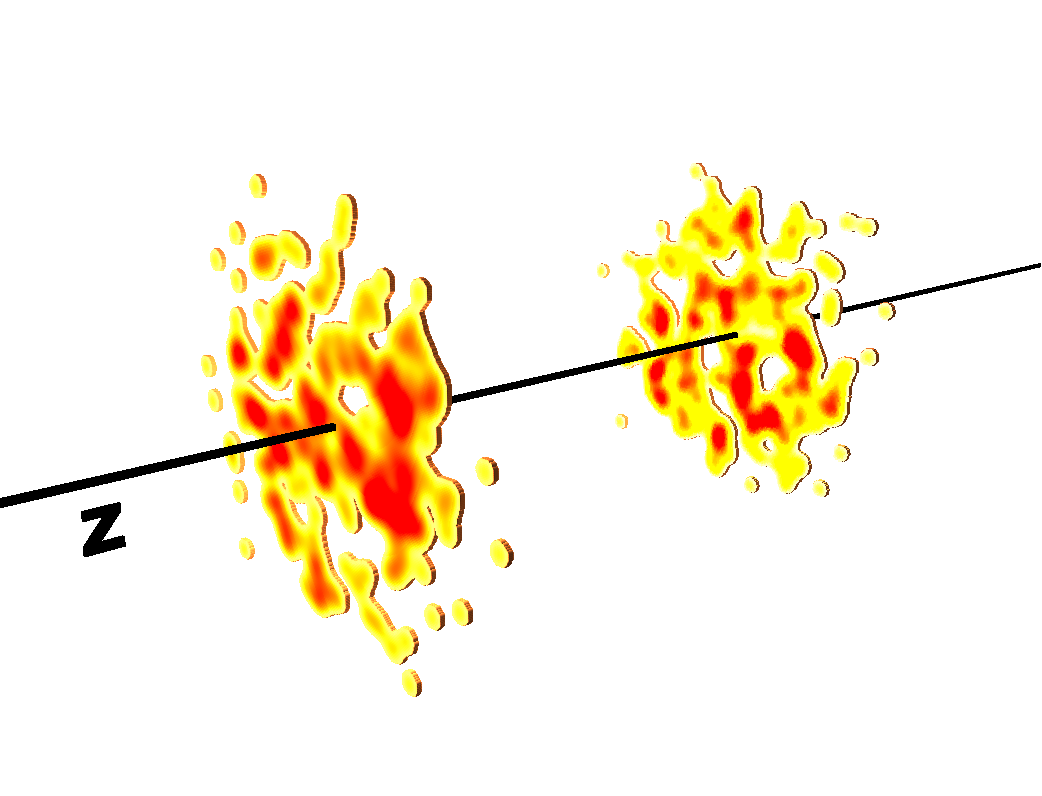
\includegraphics[width=\columnwidth]{wgmu}
 \caption{\label{fig:ipglasma} Bjorn}
\end{figure}

\subsection{Spacetime evolution}

\section{Hydrodynamic initial conditions}

\section{Hydrodynamic initial conditions}

\section{Fluid dynamic simulations}

\begin{figure}
 \includegraphics[width=0.15\columnwidth]{e2-crop} \hspace{.01\columnwidth} 
 \includegraphics[width=0.23\columnwidth]{e3-crop} \hspace{.01\columnwidth}
 \includegraphics[width=0.21\columnwidth]{e4-crop} \hspace{.01\columnwidth}
 \includegraphics[width=0.24\columnwidth]{e5-crop}\\
 \flushleft
 \vspace{-0.1in}
 \hspace{0.08\columnwidth} 2 \hspace{0.19\columnwidth} 3 \hspace{0.21\columnwidth} 4 \hspace{0.22\columnwidth} 5
 \caption{Diagrams of the second, third, fourth and fifth azimuthal Fourier harmonics. The angular resolution increases with increasing harmonic number.}
\end{figure}

\begin{figure*}[t]
  \centering
  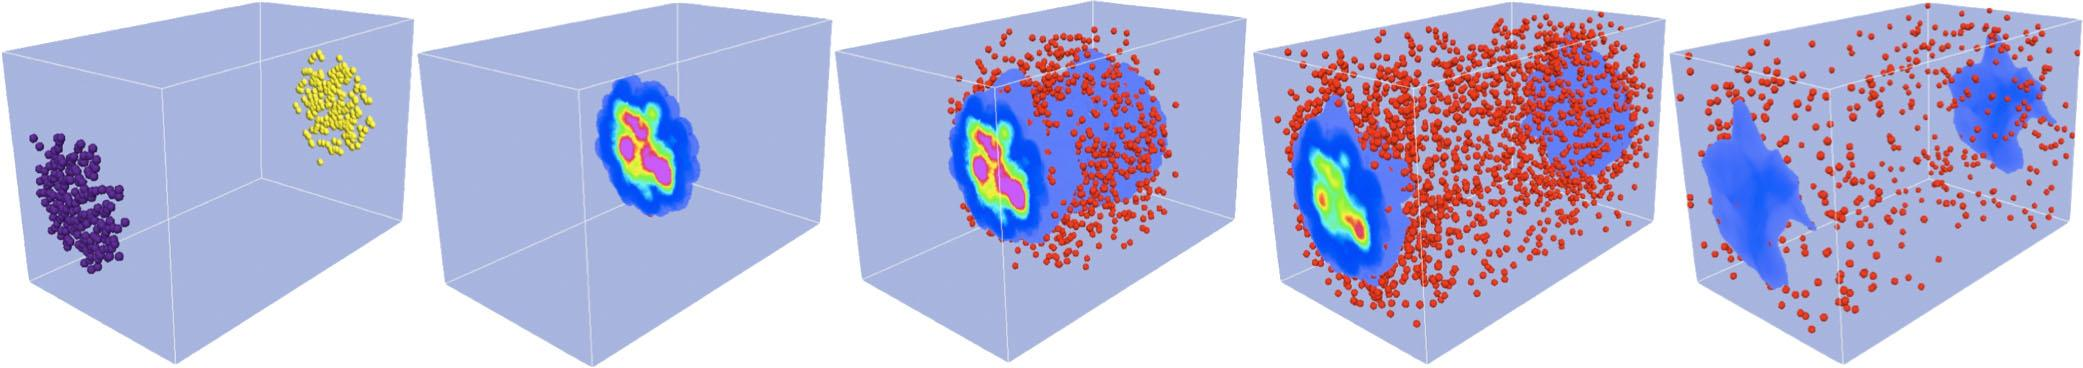
\includegraphics[width=\textwidth]{evolution} \\
  0 fm/c   \hspace{.13\textwidth}
  0.5 fm/c \hspace{.13\textwidth}
  8 fm/c   \hspace{.13\textwidth}
  16 fm/c  \hspace{.13\textwidth}
  22 fm/c
  \caption{Figure from \cite{iss}}
  \label{fig:coll}
\end{figure*}


\begin{figure}
 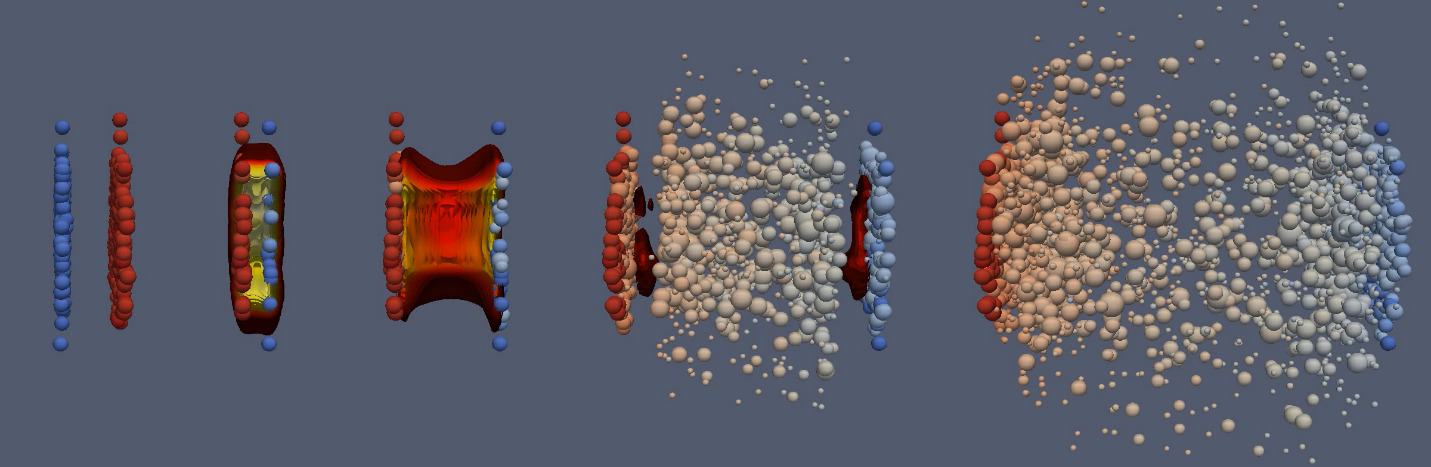
\includegraphics[width=\columnwidth]{HIC}
\end{figure}

\begin{figure*}
 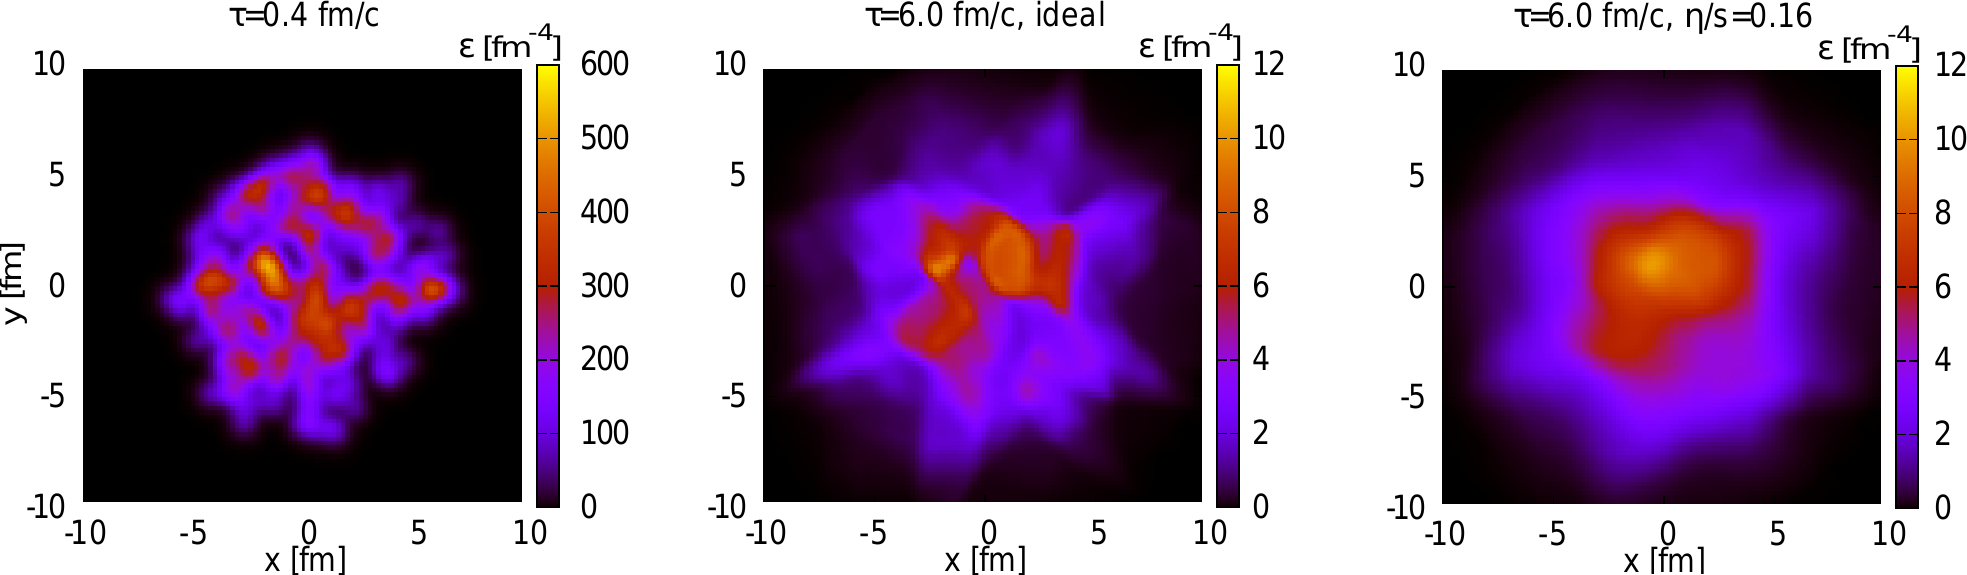
\includegraphics[width=\textwidth]{three}
\end{figure*}

\begin{figure}
 \includegraphics[height=0.19\textwidth]{motivation1-crop}\\
 \includegraphics[height=0.13\textwidth]{motivation2-crop}
\end{figure}

\begin{figure}
 \includegraphics[width=\columnwidth]{saturation}
\end{figure}

\begin{figure}
 \includegraphics[width=\columnwidth]{trento-profiles}
\end{figure}

\begin{figure*}
 \includegraphics[height=0.2\textwidth]{collision1}
 \includegraphics[height=0.2\textwidth]{collision2}
 \includegraphics[height=0.2\textwidth]{collision3}
 \includegraphics[height=0.2\textwidth]{collision4}
 \caption{\label{fig:spacetime} blah blah blah}
\end{figure*}

\begin{figure*}
 \includegraphics[width=\textwidth]{multdist}
\end{figure*}

\begin{figure*}
 \includegraphics[width=\textwidth]{eccentricity}
\end{figure*}

\bibliography{prelim,duke-qcd-refs/Duke_QCD_refs}


\end{document}
